
%(BEGIN_QUESTION)
% Copyright 2012, Tony R. Kuphaldt, released under the Creative Commons Attribution License (v 1.0)
% This means you may do almost anything with this work of mine, so long as you give me proper credit

If the rear wheel of this bicycle supports 70\% of the rider's weight, determine the compressive force within the {\it seat stays} (the struts leading from the seat of the bicycle to the center of the rear wheel, as opposed to the {\it chain stays} connecting the crank bracket to the wheel center) if the rider weighs 190 pounds.  Give your answer in the form of a total amount of compressive force for the two seat stays (there are two of them, one on each side of the rear wheel).  Assume that the chain stays are level with the ground:

$$\includegraphics[width=15.5cm]{i02579x01.eps}$$

$F_{seat stay}$ = \underbar{\hskip 50pt} lbs

\vskip 10pt

\underbar{file i02579}
%(END_QUESTION)





%(BEGIN_ANSWER)

Combined seat stay compression = {\bf 146.749 lbs}.  Ideally, this will equate to {\bf 73.37} pounds of compressive force in each of the two seat stays.

%(END_ANSWER)





%(BEGIN_NOTES)


%INDEX% Mathematics review: trigonometric calculations

%(END_NOTES)


